\pagestyle{fancy}
\section{Introducción}

AironTools es una empresa mexicana con más de una década de experiencia en la producción y comercialización de herramientas industriales. A lo largo de su trayectoria ha consolidado una base de clientes recurrentes en el sector metalmecánico y de servicios técnicos. Sin embargo, actualmente enfrenta importantes desafíos operativos derivados del uso de procesos manuales y herramientas no integradas para la gestión interna y la atención a clientes.

La gestión de servicios técnicos, inventario, comunicación interna y control de información se realiza mediante hojas de cálculo y formatos físicos, lo que ha derivado en dificultades para la trazabilidad de los servicios, errores en el registro de información, pérdida de datos importantes para la toma de decisiones, y una experiencia limitada para el cliente, al no contar con un sistema que le permita dar seguimiento a sus solicitudes de manera eficiente.

Estas deficiencias afectan directamente la eficiencia operativa, la competitividad y la capacidad de crecimiento de AironTools frente a otras empresas del sector que ya operan con sistemas digitales robustos e interconectados. En este contexto, se propone el diseño e implementación de un sistema de gestión empresarial que permita digitalizar y automatizar los procesos clave de la organización.

El objetivo del proyecto es desarrollar una plataforma integral que centralice la información, mejore la trazabilidad de los servicios ofrecidos, optimice el control de inventario y facilite la comunicación entre las distintas áreas operativas. Este sistema estará alineado con los flujos de trabajo actuales de la empresa, y se construirá bajo una arquitectura escalable que garantice su adaptabilidad y crecimiento a futuro.

Como beneficio, se espera una mejora sustancial en los tiempos de respuesta, una administración más eficiente de los recursos, una atención al cliente más ágil y profesional, y un fortalecimiento de la capacidad competitiva de AironTools en el mercado de herramientas industriales. El presente proyecto se enmarca dentro de la modalidad de experiencia profesional, y responde a una necesidad real detectada en la operación de la empresa.

\section{Justificación}

La propuesta de este proyecto surge de una necesidad concreta identificada en la operación diaria de la empresa AironTools. En la actualidad, la falta de un sistema de gestión empresarial digitalizado ha derivado en múltiples dificultades operativas, entre las que destacan una atención deficiente al cliente, escasa trazabilidad de los servicios técnicos, desorganización en el control de inventario y una gestión interna basada en registros manuales. Esta situación ha limitado significativamente la capacidad de la empresa para escalar sus operaciones y mantenerse competitiva frente a organizaciones del mismo sector que ya han implementado soluciones tecnológicas robustas.

Los registros actuales de clientes, servicios, inventario y empleados se realizan mediante formatos físicos o archivos aislados, lo cual genera errores frecuentes, pérdida de información, duplicidad de datos y demoras en la atención. Estas deficiencias impactan de manera directa en la eficiencia del personal, en la capacidad de respuesta y en la imagen profesional que la empresa proyecta a sus clientes.

Frente a este panorama, la implementación de un sistema de gestión empresarial integral representa una solución estratégica. Este sistema permitirá centralizar en una sola plataforma la información relacionada con empleados, clientes, servicios y productos, lo que facilitará la trazabilidad del flujo de trabajo desde la solicitud de un servicio hasta la entrega final. Además, la automatización de notificaciones y la digitalización de los procesos permitirán establecer una comunicación más eficiente con los clientes, otorgándoles información puntual y transparente sobre el avance de sus solicitudes.

Otra ventaja clave de esta solución es la optimización del control de inventario. A través de funciones como alertas de stock, reportes automáticos y seguimiento de movimientos, será posible reducir errores, evitar faltantes críticos y anticipar necesidades operativas. A su vez, los reportes generados por el sistema facilitarán la toma de decisiones basadas en datos reales y actualizados, incrementando la capacidad de análisis y planificación de la empresa.

En conjunto, esta propuesta tecnológica contribuirá a mejorar la productividad interna, profesionalizar la operación diaria y elevar la calidad del servicio ofrecido a los clientes. También permitirá documentar formalmente los procesos internos, asegurando su replicabilidad y continuidad. La digitalización de estas funciones no solo responde a una necesidad interna urgente, sino que posiciona a AironTools como una empresa moderna, eficiente y con visión de crecimiento sostenible en un mercado altamente competitivo.

\section{Objetivo general}
Diseñar un sistema digital de gestión empresarial para AironTools que automatice y centralice los procesos internos de atención al cliente, servicios técnicos, control de inventario y comunicación organizacional, con el fin de mejorar la eficiencia operativa, la trazabilidad de los servicios y la calidad del servicio ofrecido.

\section{Objetivos específicos}
\begin{enumerate}
	\item Desarrollar un módulo de gestión de usuarios que permita registrar, organizar y asignar roles diferenciados al personal de AironTools según sus funciones operativas.

	\item Implementar un módulo de gestión de clientes que facilite el registro, seguimiento del historial de atención y mejora en la comunicación con los clientes.

	\item Automatizar el flujo completo de los servicios técnicos, desde el ingreso del equipo hasta su entrega, integrando notificaciones en cada etapa del proceso.

	\item Diseñar un módulo de control de inventario que gestione entradas, salidas, movimientos de productos y alertas por niveles críticos de stock.
\end{enumerate}

\section{Trabajos relacionados}

A continuación se presentan seis trabajos que abordan problemáticas similares a las identificadas en el presente proyecto. Se analiza su propósito, contexto, solución implementada y resultados obtenidos, con el fin de establecer un marco de referencia que oriente el diseño del sistema propuesto para AironTools.

\subsection{Digitalización de procesos en empresas manufactureras \cite{Garcia07}}

Este proyecto terminal atendió el problema de la ineficiencia operativa en empresas manufactureras que aún empleaban procesos manuales para su gestión interna. Su objetivo fue facilitar el crecimiento empresarial mediante la digitalización de dichos procesos. La solución consistió en diseñar e implementar un sistema digital de gestión que integrara herramientas tecnológicas para mejorar el control interno. Como resultado, se logró una mayor eficiencia y trazabilidad en operaciones administrativas.

\subsection{Automatización en servicios técnicos con enfoque operativo \cite{Nin1992}}

El estudio abordó las fallas de trazabilidad y errores humanos en la atención de servicios técnicos. Para mejorar la calidad del servicio al cliente, se propuso automatizar el ciclo completo del proceso técnico. La solución consistió en aplicar sistemas computacionales que digitalizan cada etapa del servicio, desde el ingreso hasta la entrega del equipo. Se obtuvo como resultado una reducción significativa en errores y tiempos de atención.

\subsection{Transformación digital en PyMEs industriales \cite{Rodeiro2012}}

Este artículo respondió a la necesidad de pequeñas y medianas empresas industriales de mantenerse competitivas frente al avance tecnológico. Su propósito fue identificar factores clave para la adopción de tecnologías digitales en entornos de bajos recursos. La solución planteó estrategias prácticas de implementación con bajo costo y alto impacto. Los resultados mostraron un aumento en la productividad y eficiencia operativa.

\subsection{Sistemas de gestión de inventario en el sector de herramientas \cite{Flores2015}}

Esta tesis de maestría se enfocó en resolver los problemas de descontrol de stock en una cooperativa ferretera. El objetivo fue implementar un sistema digital de inventario para mejorar la visibilidad de existencias. La solución fue un software que permitía el registro en tiempo real de entradas y salidas, así como alertas por niveles críticos. Se logró reducir pérdidas y mejorar el control de recursos físicos.

\subsection{Importancia de la comunicación interna digitalizada \cite{Reyes2012}}

Este proyecto investigó la falta de coordinación entre departamentos en empresas medianas debido a comunicaciones fragmentadas. Se propuso implementar plataformas digitales de mensajería interna para mejorar la eficiencia organizacional. El estudio concluyó que la digitalización de la comunicación impacta positivamente en la productividad y en el ambiente laboral.

\subsection{Mejora de la experiencia del cliente mediante sistemas integrados \cite{Patino2019}}

Esta investigación abordó la desconexión entre áreas de atención al cliente y los procesos internos de las empresas. Su objetivo fue identificar cómo los sistemas digitales integrados pueden mejorar la experiencia del usuario. Se desarrolló una plataforma que unificaba seguimiento de servicios, notificaciones y canales de contacto. Como resultado, se observó un aumento en la fidelización y satisfacción del cliente.

\begin{longtable}{m{.05\paperwidth} *{2}{m{.33\paperwidth}} @{}}
	\caption{Comparación cualitativa de los trabajos relacionados con el proyecto.}
	\label{table:trabajosRelacionados}\\
	\hline
	\textbf{Ref.} & \textbf{Similitudes} & \textbf{Diferencias} \\
	\hline
	\endfirsthead
	
	\multicolumn{3}{c}{\textbf{Continuación de la Tabla \ref{table:trabajosRelacionados}}} \\
	\hline
	\textbf{Ref.} & \textbf{Similitudes} & \textbf{Diferencias} \\
	\hline
	\endhead
	\hline
	\endlastfoot
	
	\cite{Garcia07} &
	\begin{itemize}[topsep=0pt,itemsep=0pt,parsep=0pt,partopsep=0pt,leftmargin=*]
		\item Digitalización de procesos internos.
		\item Enfoque en eficiencia operativa.
		\item Sector industrial como contexto principal.
	\end{itemize} &
	\begin{itemize}[topsep=0pt,itemsep=0pt,parsep=0pt,partopsep=0pt,leftmargin=*]
		\item Falta de especialización en servicios técnicos.
	\end{itemize} \\
	\midrule
	
	\cite{Nin1992} &
	\begin{itemize}[topsep=0pt,itemsep=0pt,parsep=0pt,partopsep=0pt,leftmargin=*]
		\item Automatización del flujo técnico.
		\item Mejora de trazabilidad.
		\item Procesos estructurados por etapas.
	\end{itemize} &
	\begin{itemize}[topsep=0pt,itemsep=0pt,parsep=0pt,partopsep=0pt,leftmargin=*]
		\item Tecnología desactualizada.
		\item Poca atención al cliente final.
	\end{itemize} \\
	\midrule
	
	\cite{Rodeiro2012} &
	\begin{itemize}[topsep=0pt,itemsep=0pt,parsep=0pt,partopsep=0pt,leftmargin=*]
		\item Contexto PyME industrial.
		\item Adopción tecnológica gradual.
	\end{itemize} &
	\begin{itemize}[topsep=0pt,itemsep=0pt,parsep=0pt,partopsep=0pt,leftmargin=*]
		\item Escaso detalle técnico en implementación.
	\end{itemize} \\
	\midrule
	
	\cite{Flores2015} &
	\begin{itemize}[topsep=0pt,itemsep=0pt,parsep=0pt,partopsep=0pt,leftmargin=*]
		\item Gestión de inventario digital.
		\item Sector ferretero similar.
	\end{itemize} &
	\begin{itemize}[topsep=0pt,itemsep=0pt,parsep=0pt,partopsep=0pt,leftmargin=*]
		\item Alcance limitado al control de stock.
	\end{itemize} \\
	\midrule
	
	\cite{Reyes2012} &
	\begin{itemize}[topsep=0pt,itemsep=0pt,parsep=0pt,partopsep=0pt,leftmargin=*]
		\item Necesidad de comunicación interna efectiva.
		\item Uso de plataformas digitales organizacionales.
	\end{itemize} &
	\begin{itemize}[topsep=0pt,itemsep=0pt,parsep=0pt,partopsep=0pt,leftmargin=*]
		\item No implementa una solución tecnológica específica.
	\end{itemize} \\
	\midrule
	
	\cite{Patino2019} &
	\begin{itemize}[topsep=0pt,itemsep=0pt,parsep=0pt,partopsep=0pt,leftmargin=*]
		\item Mejora de experiencia del cliente.
		\item Seguimiento digital de servicios.
	\end{itemize} &
	\begin{itemize}[topsep=0pt,itemsep=0pt,parsep=0pt,partopsep=0pt,leftmargin=*]
		\item Contexto distinto (empresa propia).
	\end{itemize} \\
	\bottomrule
	\end{longtable}
	

\section{Descripción Técnica}

El sistema de gestión empresarial propuesto para AironTools está diseñado como una aplicación web moderna que permite automatizar procesos clave como la atención al cliente, la gestión de servicios técnicos, el control de inventario y la comunicación interna. Se desarrollará utilizando tecnologías actuales que aseguran escalabilidad, seguridad y mantenimiento eficiente.

\subsection{Arquitectura del Sistema}

Se utilizará una arquitectura basada en microservicios, lo cual permitirá escalar módulos de forma independiente, mejorar la tolerancia a fallos y facilitar la implementación modular. Cada servicio podrá operar de forma autónoma y comunicarse con los demás a través de APIs RESTful seguras.

\subsection{Módulos Principales del Sistema}

\begin{itemize}
	\item \textbf{Módulo de Usuarios y Roles}: Gestiona el acceso al sistema mediante autenticación y autorización. Soporta distintos perfiles (administrador, ventas, técnico, etc.).

	\item \textbf{Módulo de Clientes}: Permite registrar y consultar datos de los clientes, sus servicios activos e historial.

	\item \textbf{Módulo de Servicios Técnicos}: Controla el flujo de atención a herramientas, desde su ingreso hasta la entrega. Incluye diagnósticos, cotizaciones, reparaciones y cierre.

	\item \textbf{Módulo de Inventario}: Administra el stock de herramientas, repuestos y productos, con alertas automáticas y reportes de movimientos.

	\item \textbf{Módulo de Notificaciones}: Informa al cliente sobre el estado de sus servicios mediante correo electrónico y alertas internas. También facilita la comunicación entre empleados.
\end{itemize}

\subsection{Tecnologías Utilizadas}

\textbf{Frontend:}
\begin{itemize}
	\item \textbf{React.js} con \textbf{TypeScript} para una interfaz interactiva y mantenible.
	\item \textbf{HTML5} y \textbf{CSS3} para estructura y estilos.
	\item \textbf{Axios} para comunicación con el backend.
	\item \textbf{Figma} y \textbf{Material UI} para diseño de interfaz (UI/UX).
\end{itemize}

\textbf{Backend:}
\begin{itemize}
	\item \textbf{NestJS} con \textbf{TypeScript}, basado en arquitectura modular.
	\item \textbf{MongoDB} como base de datos no relacional por su flexibilidad.
	\item \textbf{Node.js} como entorno de ejecución.
	\item \textbf{Jest} para pruebas automatizadas.
\end{itemize}

\textbf{Otros componentes:}
\begin{itemize}
	\item \textbf{Docker} para contenedores y despliegue.
	\item \textbf{GitHub Actions} para integración y despliegue continuo (CI/CD).
	\item \textbf{Visual Studio Code} como entorno de desarrollo.
\end{itemize}








\section{Especificación Técnica}

El desarrollo del sistema de gestión empresarial para AironTools se basa en un enfoque modular, escalable y centrado en los procesos críticos de la empresa. El sistema será accesible a través de una aplicación web y podrá ser utilizado por empleados autorizados desde distintos dispositivos.

\subsection{Alcance del Proyecto}

El proyecto incluye el diseño, desarrollo e implementación de los siguientes módulos funcionales:

\begin{itemize}
	\item Registro y gestión de empleados con roles diferenciados.
	\item Registro de clientes y su historial de servicios.
	\item Gestión completa del flujo de servicios técnicos.
	\item Control del inventario de herramientas y productos.
	\item Notificaciones automáticas para empleados y clientes.
	\item Comunicación interna por mensajería o correo empresarial.
	\item Generación de reportes operativos.
\end{itemize}

Cada módulo será desarrollado, probado e integrado de forma progresiva para asegurar una implementación ordenada.

\subsection{Tecnologías y Arquitectura}

El sistema utilizará una arquitectura cliente-servidor basada en microservicios. El frontend será desarrollado en \textbf{React.js} y \textbf{TypeScript}, mientras que el backend será implementado en \textbf{NestJS} sobre \textbf{Node.js}. Para el almacenamiento de datos se usará \textbf{MongoDB}, una base de datos NoSQL flexible y escalable.

El sistema se ejecutará en contenedores mediante \textbf{Docker}, y el flujo de integración y entrega continua será gestionado con \textbf{GitHub Actions}.

\subsection{Criterio de Finalización del Proyecto}

El proyecto se considerará finalizado cuando todos los módulos definidos hayan sido desarrollados, integrados y validados mediante pruebas funcionales. Además, deberá estar documentado correctamente y desplegado en un entorno de pruebas funcional.

\begin{itemize}
	\item Todos los módulos deben cumplir con los casos de uso definidos.
	\item Debe existir documentación técnica y manual de usuario.
	\item El sistema debe estar instalado en un servidor funcional o entorno en la nube.
	\item Se debe realizar una presentación funcional ante la Coordinación.
\end{itemize}

\textbf{Figura \ref{fig:componentes-sistema}} muestra la arquitectura general del sistema, y la \textbf{Figura \ref{fig:casos-uso}} representa los principales casos de uso que deben cumplirse para la validación del proyecto.

\vspace{0.5cm}

%Este texto SÍ debe incluirse para que la propuesta pueda ser aceptada.
Al concluir el proyecto de integración se entregará a la Coordinación de Estudios de Ingeniería en Computación una carpeta digital que incluirá el reporte final del proyecto en un archivo PDF (sin restricciones)\footnote{Debe poder visualizarse sin solicitar contraseña}, el código fuente de la aplicación en un archivo comprimido (sin restricciones)\footnote{Debe poder descomprimirse sin solicitar contraseña}. Además, la sección de apéndices del reporte final contendrá al menos un listado del código fuente desarrollado.

\section{Calendario de Actividades}

El desarrollo del proyecto se llevará a cabo durante el trimestre 2025-Invierno, como parte de la UEA "Proyecto de Integración de Ingeniería en Computación I" (clave 1100113), con un valor de 18 créditos y una duración de 198 horas.

A continuación se presenta el calendario de actividades, distribuido en 10 fases principales, cada una con su respectivo número de horas y entregables.

\begin{longtable}{p{0.05\textwidth} p{0.45\textwidth} p{0.1\textwidth} p{0.30\textwidth}}
	\label{table:calendarioActividades}                                                                                                                                               \\
	\toprule
	\textbf{No.} & \textbf{Actividad}                                                           & \textbf{Horas} & \textbf{Entregable}                                                \\
	\hline
	\endfirsthead

	\hline
	\textbf{No.} & \textbf{Actividad}                                                           & \textbf{Horas} & \textbf{Entregable}                                                \\
	\hline
	\endhead

	\hline
	\caption{Listado de actividades a realizar durante el trimestre 2025-Invierno.}
	\endlastfoot

	1            & Levantamiento de requerimientos y análisis del sistema actual en AironTools. & 20             & Documento de requerimientos                                        \\
	\midrule

	2            & Diseño de arquitectura del sistema y definición de módulos.                  & 20             & Diagramas de arquitectura y diseño técnico                         \\
	\midrule

	3            & Desarrollo del módulo de autenticación y gestión de usuarios.                & 25             & Módulo funcional con control de acceso y roles                     \\
	\midrule

	4            & Desarrollo del módulo de gestión de clientes.                                & 20             & Registro, historial y vista de clientes implementados              \\
	\midrule

	5            & Desarrollo del módulo de servicios técnicos (flujo completo).                & 25             & Módulo de flujo de servicio técnico automatizado                   \\
	\midrule

	6            & Desarrollo del módulo de inventario.                                         & 20             & Registro, movimientos y alertas de inventario                      \\
	\midrule

	7            & Implementación de sistema de notificaciones y comunicación interna.          & 20             & Notificaciones por correo, alertas internas y tareas asignadas     \\
	\midrule

	8            & Pruebas funcionales e integración de los módulos.                            & 20             & Reporte de pruebas, casos de uso validados                         \\
	\midrule

	9            & Despliegue en entorno de pruebas y revisión técnica.                         & 15             & Sistema desplegado en servidor y documentación preliminar          \\
	\midrule

	10           & Documentación técnica y elaboración de manual de usuario.                    & 13             & Manual de usuario, guía de instalación y documentación del sistema \\
	\bottomrule
\end{longtable}

\footnotetext{Las actividades fueron diseñadas para cubrir el desarrollo completo del sistema propuesto durante el trimestre, incluyendo análisis, diseño, codificación, pruebas, despliegue y documentación final.}

\section{Factibilidad Técnica, Operativa y Estimación de Costos}

\subsection{Factibilidad Operativa}

La implementación del sistema de gestión empresarial presenta una alta factibilidad operativa en AironTools por las siguientes razones:

\begin{itemize}
	\item \textbf{Adaptabilidad a procesos existentes:} El sistema se diseñará según las necesidades reales y flujos actuales de la empresa.
	\item \textbf{Capacitación gradual del personal:} Se planea una estrategia progresiva de formación para cada área.
	\item \textbf{Soporte técnico disponible:} El responsable del proyecto dentro de la empresa garantizará la continuidad técnica.
	\item \textbf{Aprobación de dirección:} El proyecto cuenta con el respaldo directo del jefe de área: \textbf{Mtro. Víctor Benjamín Aguilar Orocio}.
\end{itemize}

\subsection{Factibilidad Técnica}

El proyecto es técnicamente viable debido a los siguientes elementos disponibles:

\subsubsection{Recursos de desarrollo y pruebas}
\begin{itemize}
	\item Equipos de cómputo con procesadores Intel i7, 16GB RAM y SSDs.
	\item Acceso a entornos locales y remotos para desarrollo y despliegue.
	\item Conectividad de red estable para pruebas multiusuario.
\end{itemize}

\subsubsection{Herramientas utilizadas}
\begin{itemize}
	\item \textbf{Frontend:} React.js + TypeScript, Figma, Material UI.
	\item \textbf{Backend:} NestJS, Node.js, MongoDB.
	\item \textbf{Control de versiones:} Git y GitHub.
	\item \textbf{Despliegue:} Docker, GitHub Actions.
\end{itemize}

\subsubsection{Conocimientos del desarrollador}
\begin{itemize}
	\item Experiencia en diseño de software empresarial.
	\item Conocimientos avanzados en desarrollo fullstack.
	\item Capacidad para realizar pruebas, documentación y despliegue.
\end{itemize}

\subsection{Estimación de Costos}

La siguiente tabla muestra una estimación aproximada de los costos asociados al desarrollo e implementación del sistema durante el trimestre.

\begin{longtable}{|p{0.5\textwidth}|p{0.2\textwidth}|p{0.2\textwidth}|}
	\hline
	\textbf{Rubro}                              & \textbf{Costo mensual (MXN)} & \textbf{Costo trimestral (MXN)} \\
	\hline
	\endfirsthead

	\hline
	\textbf{Rubro}                              & \textbf{Costo mensual (MXN)} & \textbf{Costo trimestral (MXN)} \\
	\hline
	\endhead

	Infraestructura de servidores y pruebas     & \$3,000                      & \$9,000                         \\
	\hline
	Licencias y servicios en la nube            & \$2,000                      & \$6,000                         \\
	\hline
	Desarrollo de software (frontend y backend) & \$25,000                     & \$75,000                        \\
	\hline
	Diseño UI/UX y prototipos                   & \$10,000                     & \$30,000                        \\
	\hline
	Capacitación y soporte al personal          & \$5,000                      & \$15,000                        \\
	\hline
	Pruebas de calidad y documentación          & \$4,000                      & \$12,000                        \\
	\hline
	\textbf{Total estimado}                     & \textbf{\$49,000}            & \textbf{\$147,000}              \\
	\hline
	\caption{Estimación de costos para el desarrollo del sistema propuesto.}
	\label{tabla:costos}
\end{longtable}

\footnotetext{Los costos fueron estimados con base en referencias de mercado y validación interna con el responsable del área. Incluyen desarrollo, pruebas, capacitación e infraestructura necesaria para el trimestre.}


\begin{figure}[H]
	\centering
	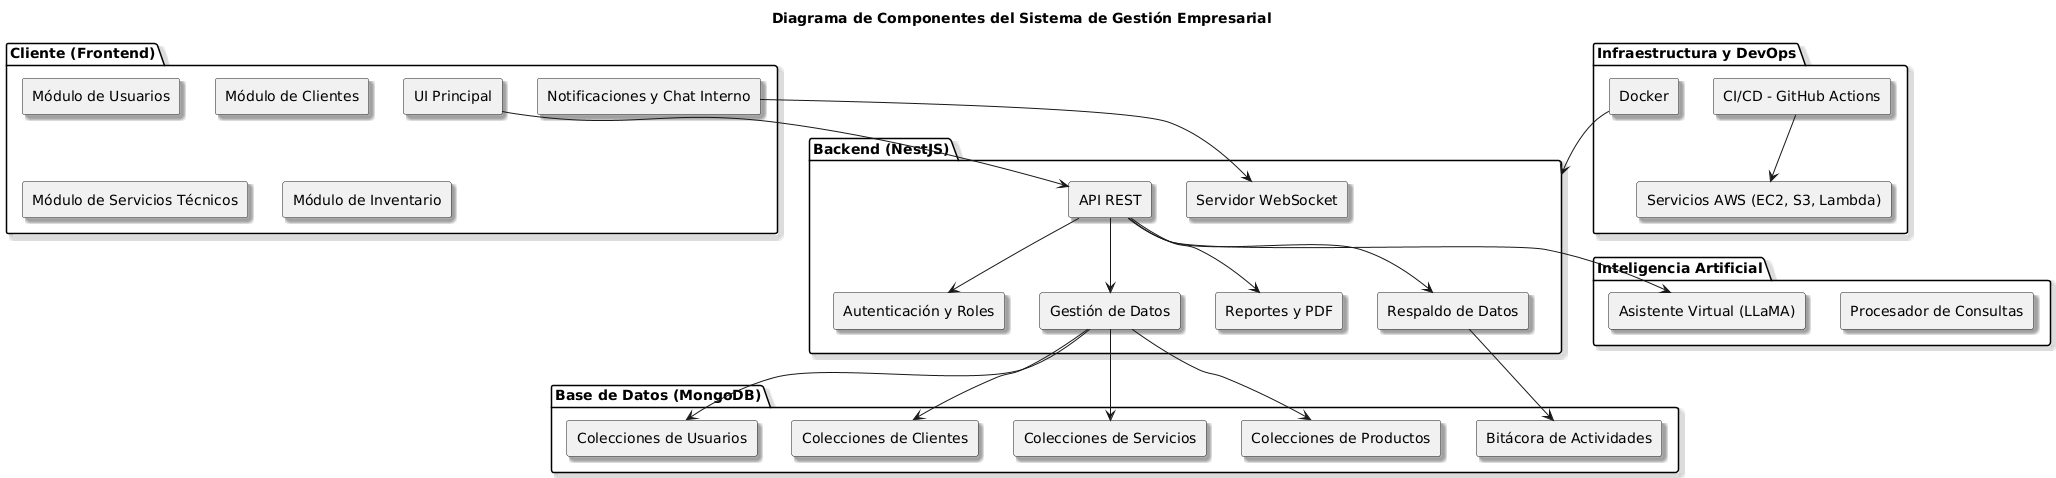
\includegraphics[width=0.8\textwidth]{componentes-sistema.png}
	\caption{Diagrama de Componentes del Sistema}
	\label{fig:componentes-sistema}
\end{figure}


\begin{figure}[H]
	\centering
	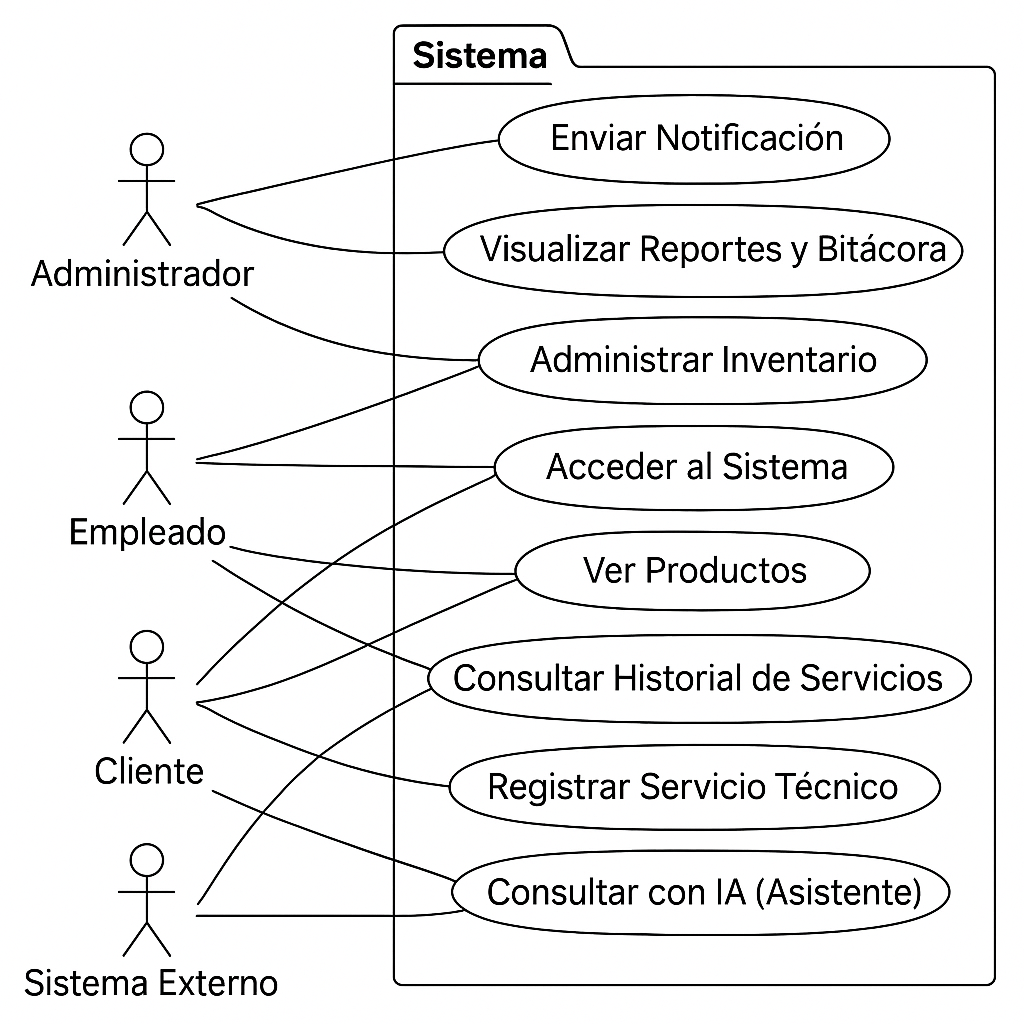
\includegraphics[width=0.8\textwidth]{casos-uso-sistema.png}
	\caption{Diagrama de Casos de Uso del Sistema}
	\label{fig:casos-uso}
\end{figure}


\begin{figure}[H]
	\centering
	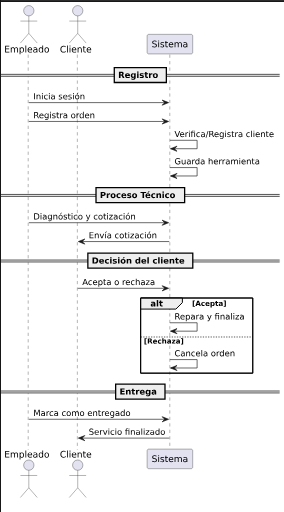
\includegraphics[width=0.8\textwidth]{secuencia-sistema.png}
	\caption{Diagrama de Secuencia del Sistema}
	\label{fig:secuencia-sistema}
\end{figure}


\begin{figure}[H]
	\centering
	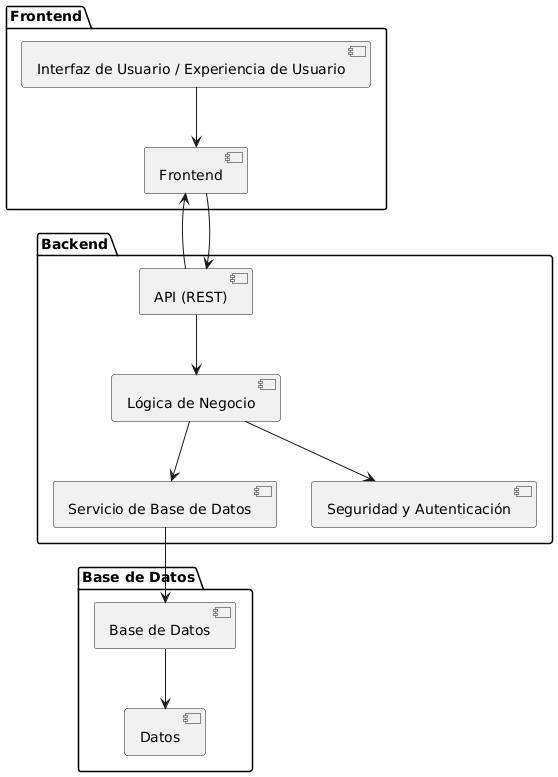
\includegraphics[width=0.8\textwidth]{sistema.png}
	\caption{Vista general del sistema propuesto}
	\label{fig:vista-general}
\end{figure}